\documentclass[a4paper,oneside,12pt,liststotoc,bibtotoc]{scrbook}


\usepackage[latin1]{inputenc}
\usepackage{ngerman}
\usepackage{scrpage2}
\usepackage{pdfpages}

\usepackage{bakk}

\usepackage{color}
\usepackage{courier}
\usepackage{graphicx}           % Grafiken
\usepackage{listings} 
          % Listings
\usepackage{bibgerm,cite}       % Deutsche Bezeichnungen, Automatisches Zusammenfassen von Literaturstellen
\usepackage[ngerman]{varioref}  % Querverweise
\usepackage{verbatim}           % Code-Umgebung
\usepackage{xspace}             % Richtige Leerzeichen f\"{u}r Makros

\usepackage{appendix}


\tolerance=4000
\emergencystretch=30pt

%% Numeriere 3 Ebenen tief (bis subsection)
\setcounter{secnumdepth}{3}
%% nimm 3 Ebenen in das Inhaltsverzeichni%s auf.
\setcounter{tocdepth}{4}



\begin{document}

% Gloabe Einstellungen f\"{u}r Listings
\lstset{
  basicstyle=\ttfamily\tiny,
  frame=single,
  xleftmargin=10pt,
  xrightmargin=10pt,
%  numbers=left,
%  breaklines=true,
  tabsize=2
%  showspaces=false
}

%************************************************************************
% Titelseite
%************************************************************************

\newcommand{\advisor}{BREITENECKER Felix, SCHNECKENREITHER G�nter}
\newcommand{\kindOfWork}{""}
\newcommand{\lva}{Simulation}
\author{BRODER J�rgen, 0425784\\
ECKER Valentin, 0426030
}

\date{\today}
\title{Simulationsprotokoll Parallelagenten}
\maketitle
\pagenumbering{roman}
\parindent0pt %Einr�cken f�r das gesamte Dokument verhindern



\newpage

\pagenumbering{arabic}

\pagestyle{scrheadings}

% Kopf- und Fu{\ss}zeilen definieren
\automark[chapter]{chapter}
\ihead[]{\headmark} % innen (links) Kapitel
\chead[]{}
\ohead[\pagemark]{\pagemark} % au{\ss}en (rechts) Seitenzahl
\setheadsepline{0.4pt}
\cfoot[]{} % keine Fu{\ss}zeile

%{\Large \sf \bfseries \"{U}bersicht} \vspace{1cm}



%************************************************************************
%INHALTSVERZEICHNIS

%************************************************************************



\includepdfset{pages=-,noautoscale}

\includepdf{parallelagenten.pdf}

\tableofcontents

\chapter{Implementierung}

\section{Grundlengende Implementierung}

Programmiersprachen: C und OpenCL\newline
Plattform: Darwin\newline
\newline
Wie bei Implementierungen mittels OpenCL �blich gliedert sich die Ausf�hrung in einen Host- und einen Target-Teil. Der Host-Teil wird wie gewohnt auf der CPU kompiliert und dann ausgef�hrt. Der Target-Code, welcher in OpenCL geschrieben ist, wird zur Laufzeit kompiliert, und dann auf das OpenCL-Device geladen und ausgef�hrt. OpenCL-Devices k�nnen sowohl CPUs als auch GPUs sein. In unserem Fall beschr�nken wir uns auf die parallele Ausf�hrung auf der GPU. Es steht uns eine Nvidia 9400M GPU zur Verf�gung, welche 16 Threads parallel ausf�hren kann. Die Implementierung unterst�tzt sowohl multithreading als auch multiple Devices (mehrere CPU-kerne oder mehre GPUs).
\newline
Der Host-Teil hat folgende Aufgaben:
\newline
\begin{itemize}
\item Initialisierung der Agenten
\item Kompilieren des OpenCL Codes
\item Allocation des OpenCL Devices
\item Kopieren der fixen Agenten in das Device Memory
\item Allocation von Target-Memory f�r bewegliche Agenten
\item Anstarten der OpenCL Execution
\item kopieren der beweglichen Agenten in das Host-Memory nach jeder Execution
\item generieren des Outputs in Form eines Bildes im ppm-format
\end{itemize}

Der Target-Teil hat folgende Aufgaben:

\begin{itemize}
\item Berechnung ob der dem thread zugewisene beweglicher Agent einen fixen Agent in Sichtweise hat
\item �nderung der aktuellen Bewegungsrichtung den Regeln folgend
\item Berechnung der neuen Position
\item Berechnung ob neue Position ausserhalb des Simulationsfeldes liegt. Wenn ja -> Abprall an der Wand.
\end{itemize}

Die Visualiserung der Simulation findet in mehreren Stufen statt. In der Host-Applikation wird nach jedem Simulationsschritt ein Bild generiert das den aktuellen Zustand mittels farbkodierter Punkte in einem Bild darstellt. Dazu wird aufgrund der Einfachkeit das simple PPM Format verwendet. Nach der Simulation werden die erzeugten ppm Bilder in das PNG-Format umgewandelt und ein Film mit HUFYU Codierung erzeugt. Wichtig bei der Wahl der Formate ist eine verlustfreie Kompression, da sonst Agenten, welche als einzelne Pixel dargestellt werden, verloren gehen k�nnten. Diese Darstellungskette wird als bash-script mithilfe von ffmpeg f�r die Codierung umgesetzt welche sowohl Einzelbilder der Simulationsschritte erzeugt als auch das Video mit der gesamten Simualtion. 


\section{Details}

Wie in \ref{fig:basic_arch} beschrieben, wird in der hier verwendeten Implementierung der eigentliche Algorithmus auf der GPU ausgef�hrt. Es wurde darauf Wert gelegt eine m�glichst universelle und erweiterbare Implementierung zu realisieren mit dem Focus auf eine gute Skalierbarkeit. Da bei dieser Aufgabenstellung zu erwarten ist, dass der Aufwand des Speichermanagementes und Speicherkopieren um einiges Zeitaufwendiger ist als die eigentliche Berechnung der Simulation wurde darauf Wert gelegt alle Speicheroperationen m�glichst schnell abzuschliessen. D.h. es wurde f�r alle Agenten der generelle GPU-Speicher verwendet und auf eine Allocation der Streaming-Speicher verzichtet welche schneller sind, aber auf 32kB limitiert sind. Weiters w�re wie schon beschrieben dadurch ein h�herer Zeitaufwand beim Speichermanagement zu erwarten was den Vorteil des schnelleren Speichers wohl zunichte machen w�rde.

Generell ist anzumerken dass die Generierung des Outputs und das Anschliessende umkodieren der Ergebnisse nach bisherigen Erfahrungen um einiges mehr Zeit in Anspruch nimmt als die Simulation selbst. Auch bei �ber 500000 beweglichen Agenten ist dies noch der Fall. Sollten l�ngere Simulationsintervalle gew�nscht werden ist es wohl als erstes Empfehlenswert nur alle N Simulationsschritte eine Ausgabe durchzuf�hren. Wenn dies nicht m�glich ist bzw. ungew�nscht kann man sich �berlegen eine Speicheroptimierung durchzuf�hren. Auch eine h�here Anzahl an fixen Agenten sollte diese Entscheidung beg�nstigen.


\begin{figure}[htb]
	\centering
		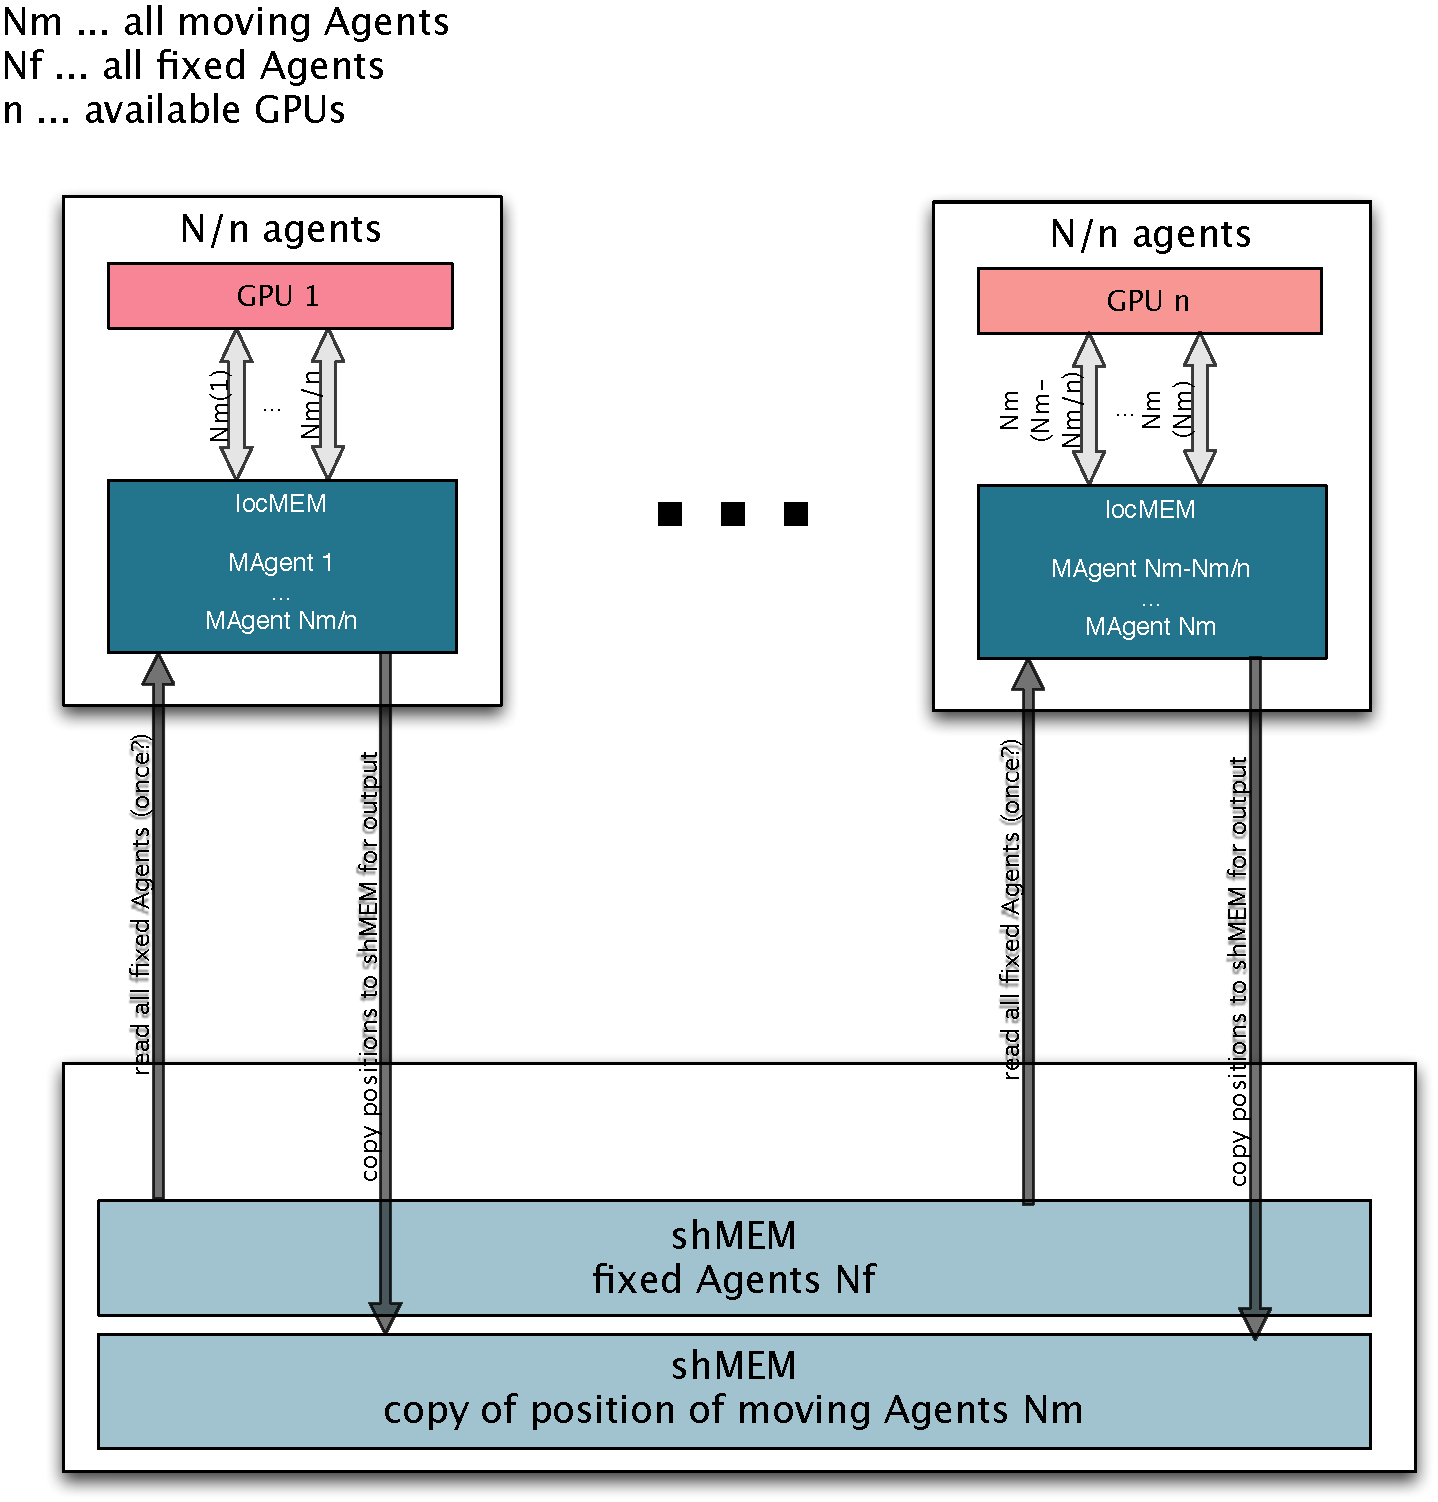
\includegraphics[width=1.0\textwidth]{chapter1/architecture.pdf}
	\caption{Basic Architecture}
	\label{fig:basic_arch}
\end{figure}

\chapter{Simulationsergebnis}


Simulationsparameter:
\begin{itemize}
\item DimX, DimY: 800x800
\item fixed agents: 12
\item fixed agents radius: DimX/6
\item moving agents: 100 000
\item moving agents initial: random position/direction
\item moving agents lookahead radius: 100
\item influence factor: 0,5
\end{itemize}

\begin{figure}[htb]
	\centering
		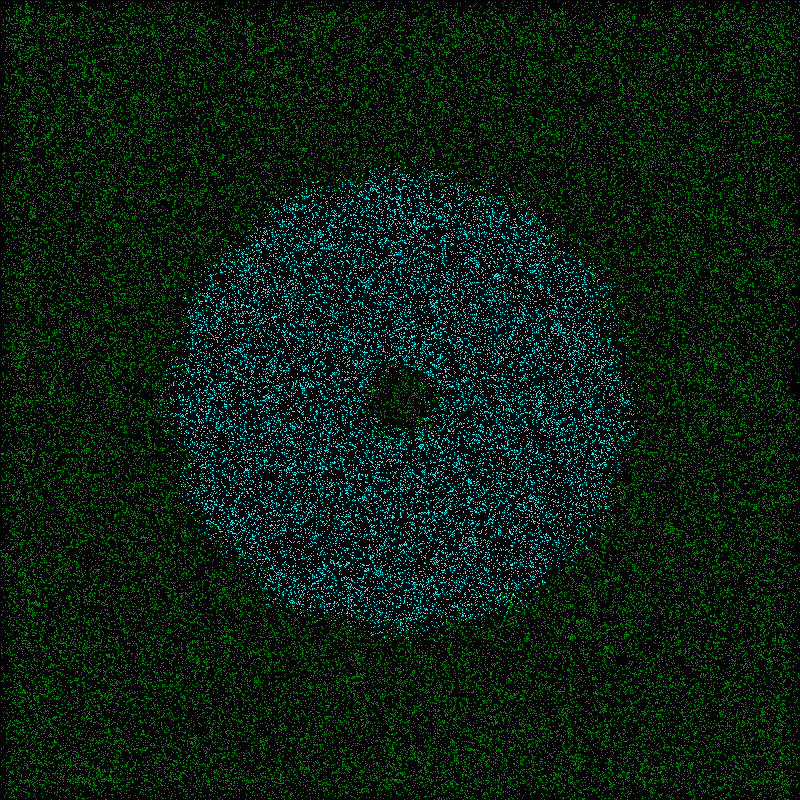
\includegraphics[width=0.9\textwidth,totalheight=0.9\textwidth]{chapter2/plot1_1.png}
	\caption{Sim1, Step 1}
	\label{fig:plot1_1}
\end{figure}

\begin{figure}[htb]
	\centering
		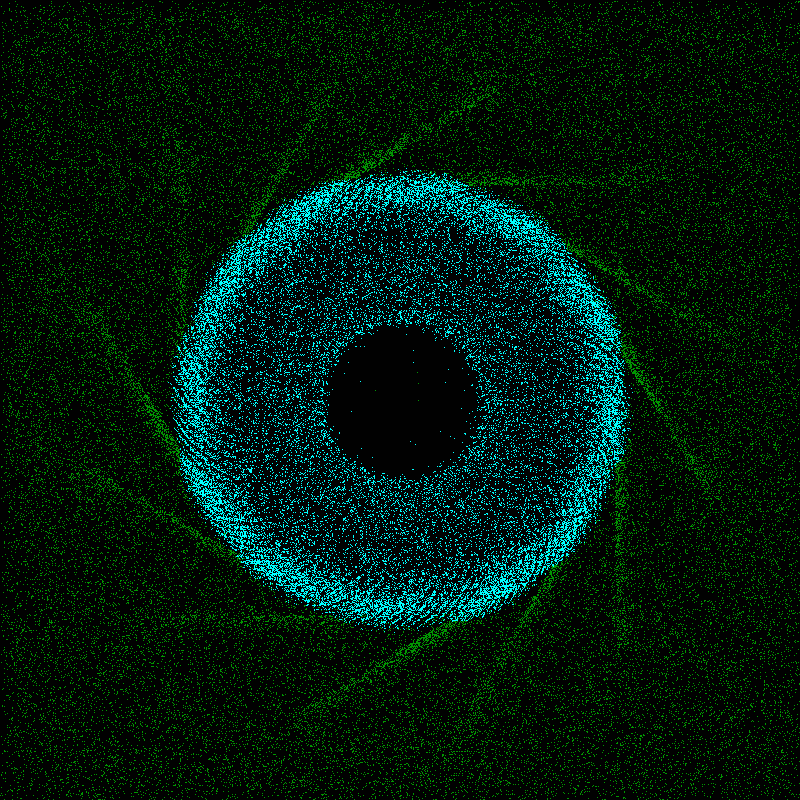
\includegraphics[width=0.9\textwidth,totalheight=0.9\textwidth]{chapter2/plot1_25.png}
	\caption{Sim1, Step 25}
	\label{fig:plot1_25}
\end{figure}

\begin{figure}[htb]
	\centering
		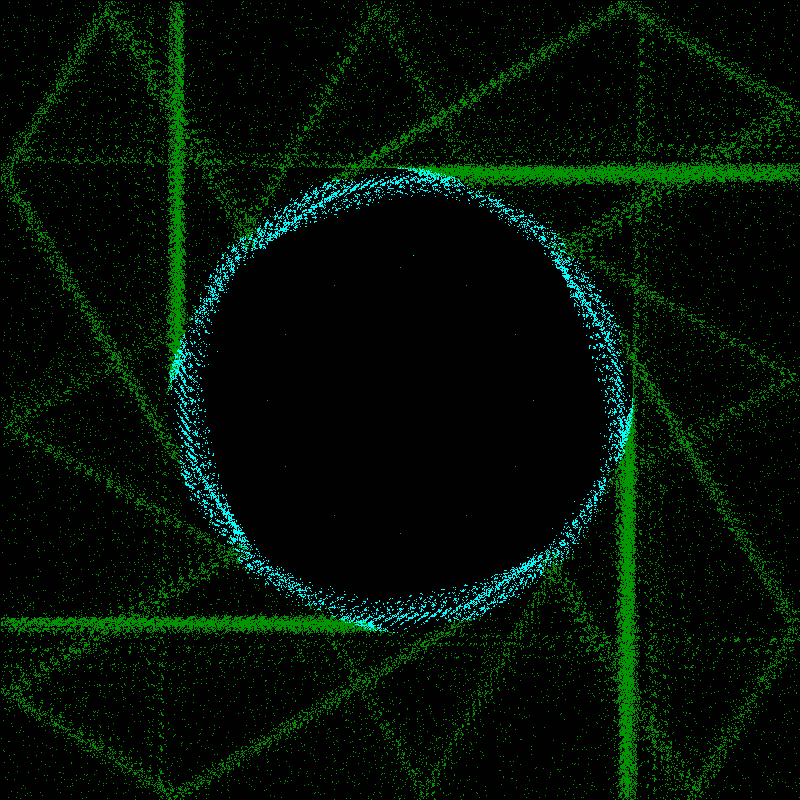
\includegraphics[width=0.9\textwidth,totalheight=0.9\textwidth]{chapter2/plot1_200.png}
	\caption{Sim1, Step200}
	\label{fig:plot1_200}
\end{figure}

\begin{figure}[htb]
	\centering
		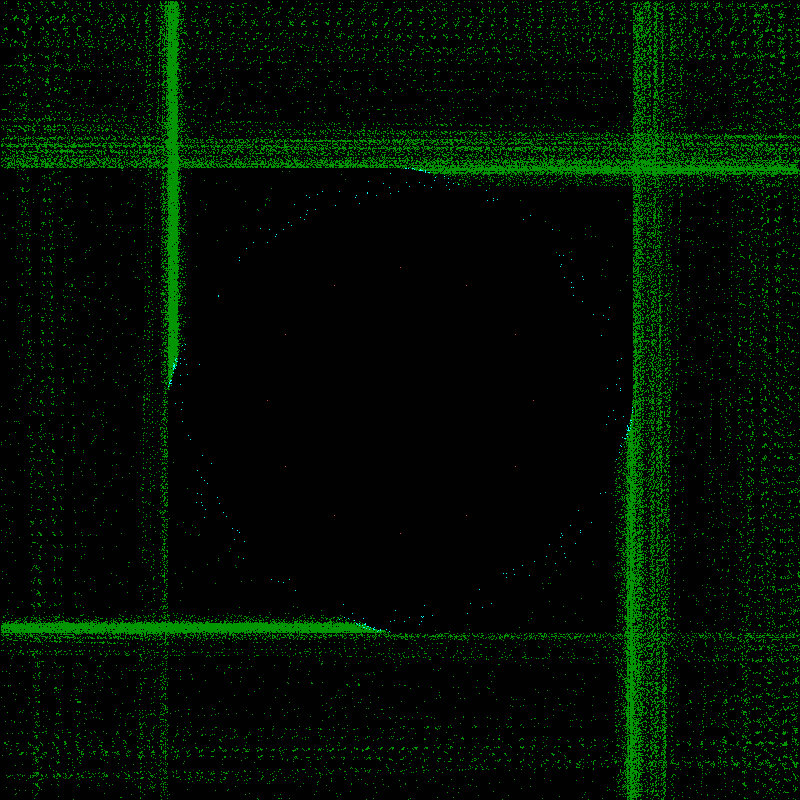
\includegraphics[width=0.9\textwidth,totalheight=0.9\textwidth]{chapter2/plot1_1000.png}
	\caption{Sim1, Step1000}
	\label{fig:plot1_1000}
\end{figure}

In Abbildung \ref{fig:plot1_1} ist die Ausgangssituation dargestellt. Zu sehen ist die zuf�llige Verteilung der beweglichen Agenten. Bewegen sich die Agenten frei, sind diese gr�n eingezeichnet, sind sie von einem fixen Agenten beeinflusst(Parameter ''moving agents lookahead radius``) sind sie t�rkis eingezeichnet. Fixe Agenten, welche die Bewegungsrichtung vorgeben, sind rot eingezeichnet. In diesem Anfangszustand mit vielen Agenten sind diese kaum erkennbar, da sie in der Zeichenebene unter den beweglichen Agenten liegen.\newline

\vspace{0.4cm}

Wie man an Abbildung \ref{fig:plot1_25} und \ref{fig:plot1_200} beobachten kann, finden sich alle beweglichen Agenten nach einer endlichen Zeit in einem Orbit um die fixen Agenten ein. Wie wir aus der Aufgabenstellung wissen, besitzen alle fixen Agenten eine Wegweiser-Vektor der normal auf dem Eigenvektor vom Mittelpunkt des Kreises steht. D.h. dass sich alle beweglichen Agenten folglich in endlicher Zeit auf den �ussersten Radius zubewegen m�ssen und diesen auch folglich irgendwann verlassen m�ssen. In Abbildung \ref{fig:plot1_200} ist gut zu erkennen wie s�mtliche beweglichen Agenten regelm��ig den ''Orbit`` verlassen um an der Aussenwand des Simulationsfeldes wieder abzuprallen. Dieses Abprallen steht so nciht in der Aufgabenstellung, und wurde von uns sinnvollerweise hinzugef�gt. Ohne dieses vorgegebene Verhalten ist zu erwarten, dass sich gegen unendlichen Simulationsverlauf alle Agenten  unendlich weit entfernen.\newline

\vspace{0.4cm}

Eine interessante Beobachtung ist auch, dass sich die Austrittspunkte aus dem Orbit immer kurz vor dem Einfluss eines im Orbit folgendem fixen Agenten befinden. Diese Beobachtung l�sst sich auch mit dem im letzten Punkt behandelten Verhalten erkl�ren, dass sich alle beweglichen Agenten immer weiter richtung �ussersten Orbit bewegen und auch am ehesten den rbit verlassen wenn die Anzahl der beinflussenden fixen Agenten am geringsten ist. Weiters ist mit fortlaufender Simulation zu beobachten dass besonders bei den in N,O,S,W stehenden fixen Agenten die beweglichen Agenten austreten bzw. h�ufen. Das ist dadurch zu erkl�ren, dass bei einer Ber�hrung der imagin�ren Wand die Agenten zur�ckgeworfen werden mit einer einfachen invertierung der kollidierenden Bewegungsrichtung. Vergleichbar auch mit einem Abprall einer Billardkugel an einer Bande. Da nun bei einem Austritt in N,O,S,W die Agenten sich auf einem fast direktem Kollisionskurs mit der begrenzenden Wand befinden, werden diese bei Erreichen auch fast direkt zur�ckgeworfen. Damit komme selbige wieder direkt in den Einfluss des gleichen fixen Agenten was in Folge wieder eine Ablenkung in die gegengesetzte Richtung gegen Wand bedeutet. Dieses Verhalten wiederholt sich bis sich der Agent im Einfluss eines anderen fixen Agenten(meistens der in Folgerichtung des Orbits) befindet, und von diesem mitabgelenkt wird. Abbildung \ref{fig:plot1_1000} best�tigt diese Theorie.
\chapter{Listings}

\section{Invoking Script}

\lstset{language=bash}
\lstinputlisting[numbers=left,breaklines]{../go.sh}

\section{Host Code}

\lstset{language=C}
\lstinputlisting[numbers=left,breaklines]{../src/oclAgents/oclAgents.cpp}

\section{Target Code}

\lstset{language=C}
\lstinputlisting[numbers=left,breaklines]{../src/oclAgents/agents.cl}

\section{shared Header}

\lstset{language=C}
\lstinputlisting[numbers=left,breaklines]{../src/oclAgents/agents.h}


\end{document}
